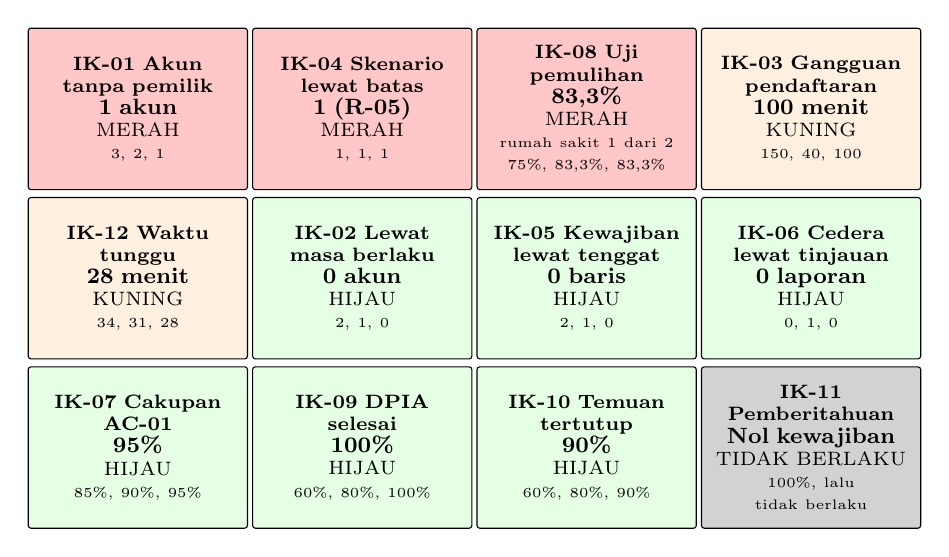
\begin{tikzpicture}[petak/.style={draw, rounded corners=1pt, align=center, text width=2.55cm, minimum height=2.05cm, font=\scriptsize, execute at begin node={\hyphenpenalty=10000}}]
  % Baris disusun dari pengecualian: merah lebih dahulu, lalu kuning, hijau, dan tidak berlaku.
  \node[petak,fill=red!22] at (0,0) {\textbf{IK-01 Akun tanpa pemilik}\\{\footnotesize\textbf{1 akun}}\\MERAH\\{\tiny\mdseries 3, 2, 1}};
  \node[petak,fill=red!22] at (2.85,0) {\textbf{IK-04 Skenario lewat batas}\\{\footnotesize\textbf{1 (R-05)}}\\MERAH\\{\tiny\mdseries 1, 1, 1}};
  \node[petak,fill=red!22] at (5.7,0) {\textbf{IK-08 Uji pemulihan}\\{\footnotesize\textbf{83,3\%}}\\MERAH\\{\tiny\mdseries rumah sakit 1 dari 2}\\{\tiny\mdseries 75\%, 83,3\%, 83,3\%}};
  \node[petak,fill=orange!12] at (8.55,0) {\textbf{IK-03 Gangguan pendaftaran}\\{\footnotesize\textbf{100 menit}}\\KUNING\\{\tiny\mdseries 150, 40, 100}};
  \node[petak,fill=orange!12] at (0,-2.15) {\textbf{IK-12 Waktu tunggu}\\{\footnotesize\textbf{28 menit}}\\KUNING\\{\tiny\mdseries 34, 31, 28}};
  \node[petak,fill=green!10] at (2.85,-2.15) {\textbf{IK-02 Lewat masa berlaku}\\{\footnotesize\textbf{0 akun}}\\HIJAU\\{\tiny\mdseries 2, 1, 0}};
  \node[petak,fill=green!10] at (5.7,-2.15) {\textbf{IK-05 Kewajiban lewat tenggat}\\{\footnotesize\textbf{0 baris}}\\HIJAU\\{\tiny\mdseries 2, 1, 0}};
  \node[petak,fill=green!10] at (8.55,-2.15) {\textbf{IK-06 Cedera lewat tinjauan}\\{\footnotesize\textbf{0 laporan}}\\HIJAU\\{\tiny\mdseries 0, 1, 0}};
  \node[petak,fill=green!10] at (0,-4.3) {\textbf{IK-07 Cakupan AC-01}\\{\footnotesize\textbf{95\%}}\\HIJAU\\{\tiny\mdseries 85\%, 90\%, 95\%}};
  \node[petak,fill=green!10] at (2.85,-4.3) {\textbf{IK-09 DPIA selesai}\\{\footnotesize\textbf{100\%}}\\HIJAU\\{\tiny\mdseries 60\%, 80\%, 100\%}};
  \node[petak,fill=green!10] at (5.7,-4.3) {\textbf{IK-10 Temuan tertutup}\\{\footnotesize\textbf{90\%}}\\HIJAU\\{\tiny\mdseries 60\%, 80\%, 90\%}};
  \node[petak,fill=gray!35] at (8.55,-4.3) {\textbf{IK-11 Pemberitahuan}\\{\footnotesize\textbf{Nol kewajiban}}\\TIDAK BERLAKU\\{\tiny\mdseries 100\%, lalu tidak berlaku}};
\end{tikzpicture}
